\documentclass{article} % For LaTeX2e
\usepackage[submission]{colm2026_conference}
\usepackage{microtype}
\usepackage{graphicx}
\usepackage{hyperref}
\usepackage{url}
\usepackage{booktabs}
\usepackage{lineno}
\usepackage{amsmath,amssymb}
\definecolor{darkblue}{rgb}{0, 0, 0.5}
\hypersetup{colorlinks=true, citecolor=darkblue, linkcolor=darkblue, urlcolor=darkblue}

\title{Behavioral Language Modeling}
\author{Anonymous authors}
\begin{document}
\ifcolmsubmission
\linenumbers
\fi
\maketitle

\begin{abstract}
% X: Objective and relevance to downstream RL.
We study which prediction targets in language-agent pretraining provide a useful initialization for downstream reinforcement learning (RL).
% Y: The action/observation distinction creates a tradeoff, not a guaranteed advantage.
Recorded interactions mix agent-generated actions with externally supplied observations, and conventional all-token causal language modeling trains on both.
It is unclear whether predicting observations helps the model learn to act or diverts capacity from learning the policy.
% Z: Formulation and concrete objective; no novelty claim for action masking itself.
We model these interactions as partially observable decision processes and formulate Behavioral Language Modeling (BLM) as autoregressive behavioral cloning over recorded agent actions.
BLM retains the full recorded history as context and restricts the next-token loss to agent-generated action spans, requiring no architectural changes or additional parameters.
% 1b: Established analytical result and its precise scope.
We derive an exact decomposition of the summed all-token loss into action, observation, and formatting terms, making explicit how joint trajectory modeling differs from policy likelihood.
% 1a: Planned empirical verification, not completed experiments.
To test the consequences for RL initialization, we specify a controlled comparison on language-agent trajectories from random initialization, holding data and training configuration fixed while changing the loss mask.
This comparison remains to be run; the formulation establishes which likelihood each objective fits, but does not establish a downstream advantage for BLM.
\end{abstract}



\section{Introduction}
% TL;DR: Interactive language agents motivate studying how pretraining targets affect later policy optimization.
Language models used as interactive agents alternate between generating text and receiving information they did not generate. A terminal agent may issue a command, read its output, and revise its next command. Interleaved reasoning and tool use makes these exchanges explicit~\citep{yao2023react}, while agentic reinforcement learning (RL) optimizes behavior across them~\citep{cheng2025agentr1}. We ask whether pretraining on agent-generated actions alone provides a better initialization for subsequent RL than predicting every token in the interaction (Figure~\ref{fig:hero}).

\begin{figure}[!t]
\centering
\begingroup
\setlength{\fboxsep}{6pt}
\setlength{\fboxrule}{0.4pt}
\fcolorbox{black!20}{white}{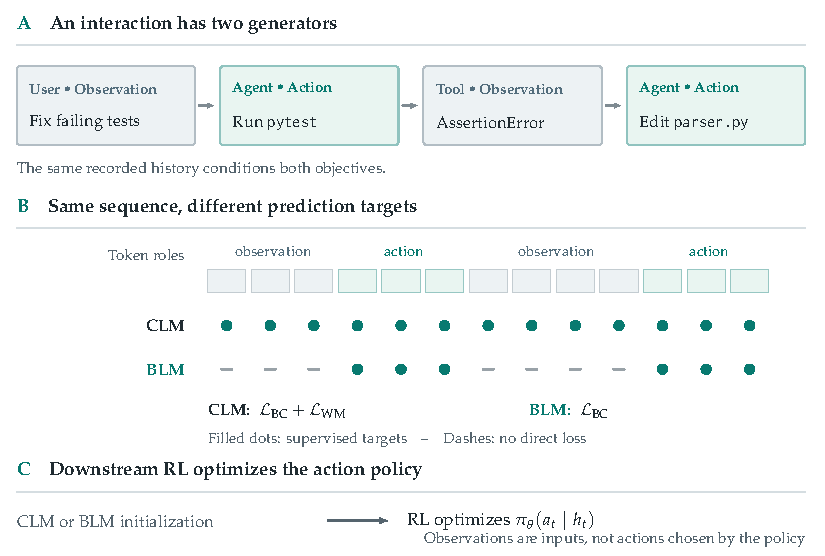
\includegraphics[width=0.88\linewidth]{hero.pdf}}
\endgroup
\caption{\textbf{Same history, different prediction targets.} CLM supervises both observations and agent actions; BLM retains observations as context and supervises actions alone. Downstream RL optimizes the action policy. The schematic loss decomposition uses summed losses and omits formatting terms; see Section~\ref{sec:method} for the full accounting.}
\label{fig:hero}
\end{figure}

% TL;DR: Token serialization preserves the distinction between agent choices and externally supplied evidence.
Consider an agent that emits \texttt{pytest}, receives \texttt{AssertionError}, and generates a patch. The command and patch are agent actions; the error is an observation supplied by the environment. We model this interaction as a partially observable Markov decision process (POMDP), using the established distinction between actions and observations~\citep{kaelbling1998planning}. Agent-generated reasoning belongs to the recorded action segment because the policy samples it, even when no external tool receives it. The boundary follows provenance and control, rather than whether a span contains natural language or code. Serializing these spans into one token sequence preserves that boundary.

% TL;DR: Action-only likelihood clones the demonstrated policy; all-token likelihood additionally models observations.
For recorded demonstrations, maximum-likelihood estimation of actions conditioned on preceding history is behavioral cloning (BC). Conventional all-token causal language modeling (CLM) additionally predicts observations and serialization tokens. With finite capacity and shared parameters, these additional targets might compete with learning the policy. They might instead improve representations of hidden state and action consequences. The difference in objectives therefore motivates an empirical comparison; it does not determine which initialization supports better downstream RL.

% TL;DR: BLM applies autoregressive BC during pretraining through an action-only loss mask.
We call the action-only pretraining objective \emph{Behavioral Language Modeling} (BLM). An autoregressive model consumes the full available recorded history, but its next-token loss covers only agent-generated action spans, including generated handoff and termination tokens. BLM changes the loss mask without adding parameters or modifying the architecture. Action masking and autoregressive BC are established techniques; our investigation concerns their use in pretraining from random initialization and their consequences for subsequent RL.

% TL;DR: A paired language-agent study tests whether the objective difference changes initial behavior and subsequent RL learning.
We specify a controlled comparison using randomly initialized Qwen3-style models and identical AgentTrove histories. The architecture, data order, optimizer, and training schedule are matched, with the loss mask as the sole intended objective change. Evaluation must distinguish policy performance immediately after pretraining from improvement during downstream RL, using initial task success and learning curves over a common environment-interaction budget. The downstream tasks, RL procedure, and evaluation budgets remain to be specified; no empirical results are available in this draft.

% TL;DR: The paper contributes explicit likelihood accounting and a controlled pretraining study, rather than a new cloning algorithm.
The paper makes the following contributions:
\begin{itemize}
\item A formulation of language-agent pretraining that separates conditional policy likelihood from joint trajectory likelihood, with exact decompositions for summed losses.
\item A token-level specification of BLM that makes action provenance, handoff boundaries, context retention, and loss normalization explicit.
\item A controlled experimental design for comparing action-only and all-token pretraining from random initialization as preparation for downstream RL.
\end{itemize}

\section{Related work}
% TL;DR: Decision Transformer and Gato establish autoregressive action prediction and selective supervision, with different conditioning and observation targets.
\paragraph{Autoregressive policy learning.}
Decision Transformer predicts actions from trajectory context and desired returns~\citep{chen2021decision}. BLM also fits autoregressive action conditionals, but does not require return conditioning; it studies the pretraining loss mask as preparation for later RL. Adding return conditioning would change the policy inputs as well as the objective under study. Gato uses selective supervision that excludes nontextual observation targets while retaining text targets~\citep{reed2022generalist}. BLM instead follows agent provenance: externally supplied text is context but not a target, while agent-generated text is supervised. These works establish that neither autoregressive BC nor selective observation masking originates here. Their complete systems change conditioning, modalities, or training data, so the matched CLM baseline isolates our loss-mask question more directly than a comparison between those systems.

% TL;DR: ActObs is the closest objective comparison; our setting changes initialization and includes prompt and framing targets in the CLM baseline.
\paragraph{Observation supervision before RL.}
ActObs directly compares action-only supervision with additional observation supervision before RL and reports benefits from the latter~\citep{zhang2026dont}. It addresses the same central question as our study. Our proposed comparison starts from random weights, whereas ActObs fine-tunes a pretrained model. The target sets also differ: ActObs keeps prompt targets masked, while our all-token CLM baseline supervises valid prompt and framing targets. CLM is therefore a joint-modeling baseline, rather than an exact reproduction of the ActObs objective. A separate condition that adds observation targets while retaining the prompt mask would be needed to isolate that objective difference. Findings from fine-tuning motivate the comparison but do not establish its outcome during pretraining from random initialization.

% TL;DR: Trajectory and world models use environmental prediction for control through mechanisms beyond direct policy imitation.
\paragraph{Predictive models for control.}
Trajectory Transformer models joint trajectories for planning~\citep{janner2021offline}, whereas BLM fits action conditionals for direct policy execution. World Models learns environmental predictions to support control~\citep{ha2018world}. These approaches motivate the possibility that observation supervision improves control, but they also change the planning procedure or model architecture. They therefore do not serve as comparisons that isolate the loss mask in our fixed policy architecture and downstream RL procedure.

\section{Background and problem setting}
\label{sec:background}
\paragraph{Interactive policies.}
% TL;DR: A POMDP has latent state $s_t$, transition kernel $T$, observation kernel $\Omega$, reward function, and an initial-state distribution.
A POMDP has latent state $s_t$, transition kernel $T$, observation kernel $\Omega$, reward function, and an initial-state distribution. At interaction step $t$, the agent has history
\begin{equation}
 h_t=(o_0,a_0,o_1,\ldots,a_{t-1},o_t),\qquad
 a_t\sim\pi_\theta(\cdot\mid h_t).
\end{equation}
The environment transitions according to $s_{t+1}\sim T(\cdot\mid s_t,a_t)$ and supplies $o_{t+1}\sim\Omega(\cdot\mid s_{t+1},a_t)$. Rewards available to the policy can be included in $o_t$. Rewards used only by the learner need not appear in its text context. Marginalizing latent state induces a history-dependent observation conditional $q(o_{t+1}\mid h_t,a_t)$. The use of histories is standard~\citep{kaelbling1998planning}. A Transformer is not assumed to compute an exact belief state.

% TL;DR: Here $a_t$ denotes the complete agent-generated segment up to the next external observation or termination.
Here $a_t$ denotes the complete agent-generated segment up to the next external observation or termination. It can contain reasoning, commands, tool-call arguments, or a final response. A deterministic interface decodes the externally executed part of this segment. Reasoning that only changes the agent's context can equivalently be viewed as an internal action with a null external transition. We model the recorded segment jointly, rather than equating each of its tokens with a separate environment step. Consecutive external messages can be grouped into one observation. We assume a fixed interface and reliable provenance labels for a single controlled agent.

\paragraph{Autoregressive action representation.}
% TL;DR: Let $a_t=(u_{t,1},\ldots,u_{t,K_t})$ be a token sequence whose terminal token or suffix marks a handoff or termination under the interface.
Let $a_t=(u_{t,1},\ldots,u_{t,K_t})$ be a token sequence whose terminal token or suffix marks a handoff or termination under the interface. We represent interaction histories as token sequences with explicit role and message boundaries, preserving temporal order. The action probability factors as
\begin{equation}
 \pi_\theta(a_t\mid h_t)
 =\prod_{k=1}^{K_t}p_\theta\bigl(u_{t,k}\mid
 h_t,u_{t,<k}\bigr).
 \label{eq:action}
\end{equation}
Fixed framing supplied before generation is part of the conditioning prefix. We assume the generation protocol defines a proper distribution over completed segments, for example by termination almost surely or an explicit length-limit rule. The autoregressive factorization describes a distribution over recorded agent outputs. Different outputs can decode to the same external command. It is this output distribution that BC fits.

\paragraph{Behavioral cloning.}
% TL;DR: Let $\mathcal D$ be a distribution over finite recorded trajectories from behavior policy $\beta$, potentially a mixture of demonstrators.
Let $\mathcal D$ be a distribution over finite recorded trajectories from behavior policy $\beta$, potentially a mixture of demonstrators. Maximum-likelihood imitation minimizes
\begin{equation}
 \mathcal L_{\mathrm{BC}}(\theta)
 =-\mathbb E_{\tau\sim\mathcal D}\sum_{t=0}^{T(\tau)-1}
 \log\pi_\theta(a_t\mid h_t).
 \label{eq:bc}
\end{equation}
No optimality of $\beta$ is assumed. This objective fits behavior under demonstrated histories. It does not solve the distribution shift that arises when the learned policy visits new histories~\citep{ross2011reduction}. Return conditioning, as in Decision Transformer~\citep{chen2021decision}, is a separate modeling choice and is not required here.

\paragraph{Serialized trajectories.}
% TL;DR: Let $x_{1:N}$ denote the token sequence representing a recorded trajectory $\tau$.
Let $x_{1:N}$ denote the token sequence representing a recorded trajectory $\tau$. Partition its token indices into agent-generated targets $\mathcal A$, observation content $\mathcal O$, and fixed formatting $\mathcal F$. These labels come from the interaction interface, not from the lexical content of a token. In particular, an agent's quoted error message is still agent-generated. A role label inserted by the serializer is framing, while a tool name or recipient selected by the policy is action content. All three types can occur in the causal input prefix.

\section{Behavioral Language Modeling}
\label{sec:method}
\subsection{Policy likelihood and joint trajectory likelihood}
% TL;DR: For clarity, first consider a fixed horizon $T$ with a final observation, $\tau=(o_0,a_0,\ldots,a_{T-1},o_T)$.
For clarity, first consider a fixed horizon $T$ with a final observation, $\tau=(o_0,a_0,\ldots,a_{T-1},o_T)$. Its distribution under the behavior policy factors as
\begin{equation}
 P_\beta(\tau)=q_0(o_0)\prod_{t=0}^{T-1}
 \beta(a_t\mid h_t)q(o_{t+1}\mid h_t,a_t).
 \label{eq:trajectory}
\end{equation}
For variable horizons, termination must be represented by an agent stop decision or environment termination event with the corresponding likelihood factor. A record ending after its last action simply lacks a final-observation factor. Exogenous recording cutoffs must not be relabeled as agent stop decisions.

% TL;DR: An autoregressive model can parameterize an analogous joint distribution $P_\theta$, using shared parameters for an action conditional $\pi_\theta$ and an observation conditional $q_\theta$.
An autoregressive model can parameterize an analogous joint distribution $P_\theta$, using shared parameters for an action conditional $\pi_\theta$ and an observation conditional $q_\theta$. On a role-delimited serialization, the two conditionals are products of next-token probabilities over their respective spans, with stopping rules that define normalized segment distributions. This does not assert that the environment depends on $\theta$. The conditional $q_\theta$ estimates an environmental distribution from data. For a serialization without additional framing targets, negative log likelihood gives the exact identity
\begin{align}
 \mathcal L_{\mathrm{CLM}}
 &= -\mathbb E_{\mathcal D}\log P_\theta(\tau)
 =\mathcal L_{\mathrm{BC}}+\mathcal L_{\mathrm{WM}},\label{eq:decomposition}\\
 \mathcal L_{\mathrm{WM}}
 &= -\mathbb E_{\mathcal D}\left[\log q_{\theta,0}(o_0)
 +\sum_{t=0}^{T-1}\log q_\theta(o_{t+1}\mid h_t,a_t)\right].
\end{align}
We call $\mathcal L_{\mathrm{WM}}$ the world-modeling loss. It predicts observations conditioned on interaction history using the same autoregressive model, without introducing a separate world model or explicit latent-state dynamics. This identity uses unnormalized sums and the same trajectory measure on both sides. Conditioning on an initial prompt removes its likelihood term. Predicting fixed framing adds its own term. Arbitrary serialized records therefore require the token-level accounting below rather than an unqualified equality between differently normalized losses.

\subsection{An action-only next-token objective}
% TL;DR: Substituting Equation~\ref{eq:action} into Equation~\ref{eq:bc} yields BLM
Substituting Equation~\ref{eq:action} into Equation~\ref{eq:bc} yields BLM
\begin{equation}
 \boxed{\mathcal L_{\mathrm{BLM}}(\theta)
 =-\mathbb E_{\tau\sim\mathcal D}\sum_{t=0}^{T(\tau)-1}
 \log\pi_\theta(a_t\mid h_t).}
 \label{eq:blm}
\end{equation}
For the concrete serialization, define $m_j=1$ if $j\in\mathcal A$ and $m_j=0$ otherwise. We use the first token $x_1$ as an unscored initial prefix, with no added beginning-of-sequence target, and require that no action starts there. Thus
\begin{equation}
 \ell_{\mathrm{BLM}}(\theta;x)
 =-\sum_{j=2}^{N}m_j\log p_\theta(x_j\mid x_{1:j-1}).
 \label{eq:token}
\end{equation}
The input vector is $(x_1,\ldots,x_{N-1})$, the target vector is $(x_2,\ldots,x_N)$, and the loss weight at input position $i$ is $m_{i+1}$. Masking by the input token's role would mislabel transitions between spans. The last recorded token $x_N$ is a target, and there is no prediction beyond the record. Padding has zero weight. Records are processed independently with a reset at their beginning. If records are packed, attention and prediction targets must not cross record boundaries.

% TL;DR: All-token CLM replaces $m_j$ by $1$ at every valid target.
All-token CLM replaces $m_j$ by $1$ at every valid target. With $\ell_S=-\sum_{j\in S\cap\{2,\ldots,N\}}\log p_\theta(x_j\mid x_{<j})$, the exact serialized identity is
\begin{equation}
 \ell_{\mathrm{CLM}}=\ell_{\mathcal A}+\ell_{\mathcal O}+\ell_{\mathcal F},
 \qquad \ell_{\mathrm{BLM}}=\ell_{\mathcal A}.
 \label{eq:serialized}
\end{equation}
Here initial prompt content is included in $\mathcal O$, and formatting targets account explicitly for deviations from Equation~\ref{eq:decomposition}.

\paragraph{Boundaries and handoffs.}
% TL;DR: A policy-generated end-of-turn, tool-handoff, or final-stop token is an action target.
A policy-generated end-of-turn, tool-handoff, or final-stop token is an action target. Otherwise the learner would fit what to emit without fitting when to return control. An end marker terminating a tool or user message is observation-side framing and is masked in BLM. Headers deterministically inserted before an assistant begins are also masked. If the interface asks the model to generate a header or choose a recipient, those generated tokens must instead be supervised. Neither a forced length cutoff nor the end of a data file creates a policy target.

\paragraph{Normalization.}
% TL;DR: For a minibatch $\mathcal B$, let $v_{b,i}$ indicate a valid within-record next-token pair, and let $w_{b,i}=v_{b,i}m_{b,i+1}$ for BLM or $w_{b,i}=v_{b,i}$ for CLM.
For a minibatch $\mathcal B$, let $v_{b,i}$ indicate a valid within-record next-token pair, and let $w_{b,i}=v_{b,i}m_{b,i+1}$ for BLM or $w_{b,i}=v_{b,i}$ for CLM. The implemented mean loss is
\begin{equation}
 \widehat{\mathcal L}_{w}
 =\frac{-\sum_{b,i} w_{b,i}\log p_\theta(x_{b,i+1}\mid x_{b,1:i})}
 {\max(1,\sum_{b,i}w_{b,i})}.
 \label{eq:batch}
\end{equation}
This is a supervised-token mean within each batch, not a mean of per-trajectory means. A batch with no targets contributes zero loss. The corpus sum in Equation~\ref{eq:blm} and its corpus-wide action-token mean differ only by a parameter-independent constant. Batch-dependent denominators can additionally change stochastic update weighting. We state the batch convention explicitly and do not apply the additive decomposition to separately normalized means. For a fixed batch with nonempty partitions, the CLM mean is instead the count-weighted average of their mean losses.

\subsection{Conditioning and downstream policy optimization}
% TL;DR: The mask changes targets, not the causal attention pattern.
The mask changes targets, not the causal attention pattern. When an action follows a tool response, its likelihood depends on the response tokens. Gradients from that action can flow through the response's embeddings and contextual computation into shared parameters. BLM therefore trains representations of observations through their usefulness for predicting subsequent actions, without directly training their generative likelihood. There is no gradient detachment at observation boundaries and no separate observation model.

% TL;DR: The relation to downstream RL follows from the same trajectory factorization.
The relation to downstream RL follows from the same trajectory factorization. For a fixed environment, trajectory log likelihood contains policy-dependent action terms and environment terms independent of policy parameters. A likelihood-ratio policy gradient for expected return $J(\theta)$ consequently has the form
\begin{equation}
 \nabla_\theta J(\theta)
 =\mathbb E_{\tau\sim P_{\pi_\theta}}\left[
 \sum_t\nabla_\theta\log\pi_\theta(a_t\mid h_t)\,G_t\right],
 \label{eq:pg}
\end{equation}
For $J(\theta)=\mathbb E[\sum_{k=0}^{T-1}\gamma^k r_k]$, the weight here is $G_t=\sum_{k=t}^{T-1}\gamma^k r_k$, with discount measured from the episode origin. Equation~\ref{eq:action} expands each score into token scores. It does not require assigning separate environment rewards to each token. Externally sampled observations have no policy score term. An observation-prediction loss can still be added deliberately as an auxiliary objective, but it is distinct from this likelihood-ratio estimator.

% TL;DR: BLM aligns the support of the supervised targets with that of policy optimization.
BLM aligns the support of the supervised targets with that of policy optimization. It does not align the entire learning problem. BC uses demonstrated histories and imitation targets, whereas RL uses policy-induced histories and rewards. It also provides no guarantee that its gradients yield more useful representations than joint training. Shared output parameters do not, by themselves, force a model to confuse speaking with observing. Causal prefixes can distinguish roles. The proposed capacity competition and behavioral biases are empirical hypotheses, balanced by the possibility that observation prediction improves consequence modeling.

\section{Experimental setup}
\label{sec:experiments}
\subsection{Language-agent comparison}
% TL;DR: The planned study uses a Qwen3-style decoder-only Transformer~\citep{yang2025qwen3}, initialized from random weights, and AgentTrove interaction records~\citep{openthoughts2026agenttrove}.
The planned study uses a Qwen3-style decoder-only Transformer~\citep{yang2025qwen3}, initialized from random weights, and AgentTrove interaction records~\citep{openthoughts2026agenttrove}. CLM and BLM will receive identical token sequences, record selection, context lengths, and sampling order, with matched initialization, architecture, optimizer, and training schedule. The mask in Equation~\ref{eq:batch} is the sole intended objective change. Unlike ActObs, whose prompt targets remain masked, the all-token CLM baseline also supervises valid prompt and framing targets. This distinction must be retained when comparing findings. We will report both allocated input positions and supervised target counts. Matching sequences does not match the number of supervised tokens, and sparse loss targets do not remove the cost of processing their context. The comparison is planned, not an account of completed training or evaluation.

% TL;DR: We preserve each retained recorded interaction and its preceding history.
We preserve each retained recorded interaction and its preceding history. With a finite context window, the current preparation retains whole records that fit and excludes overlength records rather than training isolated fragments. This changes the eligible population and must be reported. A complete record need not be a successful or complete upstream episode. Generalization to longer interactions and downstream RL remains to be measured. If future training truncates histories, the fitted policy becomes conditional on that truncated context, and the full-history interpretation must be qualified accordingly.


% TL;DR: For the planned AgentTrove comparison, the current serializer prepends a fixed ChatML role header to each message and appends \texttt{<|im\_end|>} and a newline to its body.
For the planned AgentTrove comparison, the current serializer prepends a fixed ChatML role header to each message and appends \texttt{<|im\_end|>} and a newline to its body. BLM supervises assistant bodies, including that end marker and trailing newline. Headers and non-assistant bodies are masked. The scored newline is treated as part of the demonstrated output segment, so a matching deployment protocol must let the policy generate this suffix before transferring control. If deployment instead inserts the newline deterministically after stopping at the end marker, its target must be masked to recover exactly the deployed policy likelihood. The adapter must also interpret an assistant end marker as a handoff or final stop using the interaction protocol. This serialization does not establish that an upstream recorded ending was a voluntary stop. Provenance and termination semantics require auditing. In particular, control boundaries must not be inferred solely from whether text mentions a tool.

% TL;DR: The objective requires reliable action provenance, faithful ordering, and a serialization consistent with deployment.
The objective requires reliable action provenance, faithful ordering, and a serialization consistent with deployment. It does not identify hidden agent reasoning absent from the record, infer whether demonstrations are optimal, or supply action labels for undifferentiated web text. Our use of \emph{pretraining} refers specifically to initial training on interaction demonstrations. BLM is standard autoregressive BC applied at that stage. The investigation concerns its consequences for subsequent RL, not the invention of action masking or a general argument against learning environmental dynamics.

\section{Results and discussion}
\label{sec:results}
% TL;DR: No training or downstream evaluation results are available in this draft.
No training or downstream evaluation results are available in this draft. The likelihood decomposition is an analytical result about the objectives, not evidence of an empirical advantage. The completed study must compare CLM and BLM under the setup above and report uncertainty, pretraining performance, downstream learning curves, and the training budgets and hyperparameter selection procedures needed to assess fairness.

% TL;DR: The formulation also has practical limits.
The formulation also has practical limits. Action labels require reliable provenance, finite context changes the history available to the policy, and loss normalization affects stochastic update weighting. Any findings apply to the evaluated models, interaction data, and downstream tasks; broader generalization requires further evaluation.

\section{Conclusion}
% TL;DR: We formulate language-agent pretraining through the distinction between policy actions and environmental observations.
We formulate language-agent pretraining through the distinction between policy actions and environmental observations. BLM fits demonstrated action conditionals while retaining observations as context; all-token CLM additionally fits observation and framing targets. This distinction yields explicit likelihood identities and an experimental question about initialization for subsequent RL. The current draft specifies the objectives and comparisons. Whether action-only pretraining improves downstream learning remains an empirical question.

\bibliography{main}
\bibliographystyle{colm2026_conference}
\end{document}